%%%%%%%%%%%%%%%%%%%%%%%%%%%%%%%%%%%%%%%%%%  不使用 authblk 包制作标题  %%%%%%%%%%%%%%%%%%%%%%%%%%%%%%%%%%%%%%%%%%%%%%
%-------------------------------PPT Title-------------------------------------
\title{\rm{Transformer: NLP}的新范式}
%-----------------------------------------------------------------------------

%----------------------------Author & Date------------------------------------
\author[]{\vskip +10pt 姜\;\;骏\inst{}} %[]{} (optional, use only with lots of authors)
%% - Give the names in the same order as the appear in the paper.
%% - Use the \inst{?} command only if the authors have different
%%   affiliation.
\institute[BCC]{\inst{}%
%\institute[Gain~Strong]{\inst{}%
\vskip -15pt 北京市计算中心}
%\vskip -20pt {\large 格致斯创~科技}}
\date[\today] % (optional, should be abbreviation of conference name)
{	{\fontsize{6.2pt}{4.2pt}\selectfont{\textcolor{blue}{E-mail:~}\url{jiangjun@bcc.ac.cn}}}
\vskip 45 pt {\fontsize{8.2pt}{6.2pt}\selectfont{%清华大学\;\;物理系% 报告地点
	\vskip 5 pt \textrm{2025.02}}}
}

%% - Either use conference name or its abbreviation
%% - Not really information to the audience, more for people (including
%%   yourself) who are reading the slides onlin%%   yourself) who are reading the slides onlin%%   yourself) who are reading the slides onlineee
%%%%%%%%%%%%%%%%%%%%%%%%%%%%%%%%%%%%%%%%%%%%%%%%%%%%%%%%%%%%%%%%%%%%%%%%%%%%%%%%%%%%%%%%%%%%%%%%%%%%%%%%%%%%%%%%%%%%%

\subject{}
% This is only inserted into the PDF information catalog. Can be left
% out.
%\maketitle
\frame
{
%	\frametitle{\fontsize{9.5pt}{5.2pt}\selectfont{\textcolor{orange}{“高通量并发式材料计算算法与软件”年度检查}}}
\titlepage
}
%-----------------------------------------------------------------------------

%------------------------------------------------------------------------------列出全文 outline ---------------------------------------------------------------------------------
\section*{}
\frame[allowframebreaks]
{
	\frametitle{\textrm{Outline}}
%  \frametitle{\textcolor{mycolor}{\secname}}
  \tableofcontents%[current,currentsection,currentsubsection]
}
%在每个section之前列出全部Outline
%类似的在每个subsection之前列出全部Outline是\AtBeginSubsection[]
%\AtBeginSection[]
%{
%  \frame<handout:0>%[allowframebreaks]
%  {
%    \frametitle{Outline}
%%全部Outline中,本部分加亮
%    \tableofcontents[current,currentsection]
%  }
%}

%-----------------------------------------------PPT main Body------------------------------------------------------------------------------------
\small
\section{传统的神经网络}
\begin{frame}
	\frametitle{\textrm{RNN}在\textrm{NLP}中的基本思想}
	\textcolor{purple}{循环神经网络~\textrm{(Recurrent Neural Network,~RNN)}}
    \begin{itemize}
		\setlength{\itemsep}{10pt}
    \item 序列建模:~将文本看作由单词组成的序列,\textrm{RNN}通过循环结构逐词处理,每个时间步更新隐藏状态,基于此保存文本的上下文信息\\
	    {\fontsize{7.2pt}{6.2pt}\selectfont{隐藏状态不仅受当前单词影响,还依赖之前单词的信息,借此模拟人类语言理解过程中的记忆功能}}
    \item 典型应用:~在文本生成任务中,\textrm{RNN}基于已生成的单词,不断更新隐藏状态,预测下一个单词\\
	    {\fontsize{7.2pt}{6.2pt}\selectfont{以机器翻译为例,在将源语言翻译为目标语言时,\textrm{RNN}编码器逐词处理源语言文本,生成包含语义信息的隐藏状态;~解码器再基于这些隐藏状态,逐个生成目标语言单词}}
    \end{itemize}
    \textcolor{blue}{\textrm{RNN}:~循环结构处理序列数据,每个时刻的隐藏状态不仅依赖当前输入,还依赖上一时刻的隐藏状态}\\
    \vskip 2pt
    {\fontsize{8.2pt}{6.2pt}\selectfont{这种设计使得\textrm{RNN}理论上可以捕捉长距离依赖关系,但\textrm{RNN}的循环结构决定了其计算必须按顺序进行}}
\end{frame}

\begin{frame}
	\frametitle{\textrm{RNN}在\textrm{NLP}中的基本思想}
\begin{figure}[h!]
\vspace*{-0.05in}
\centering
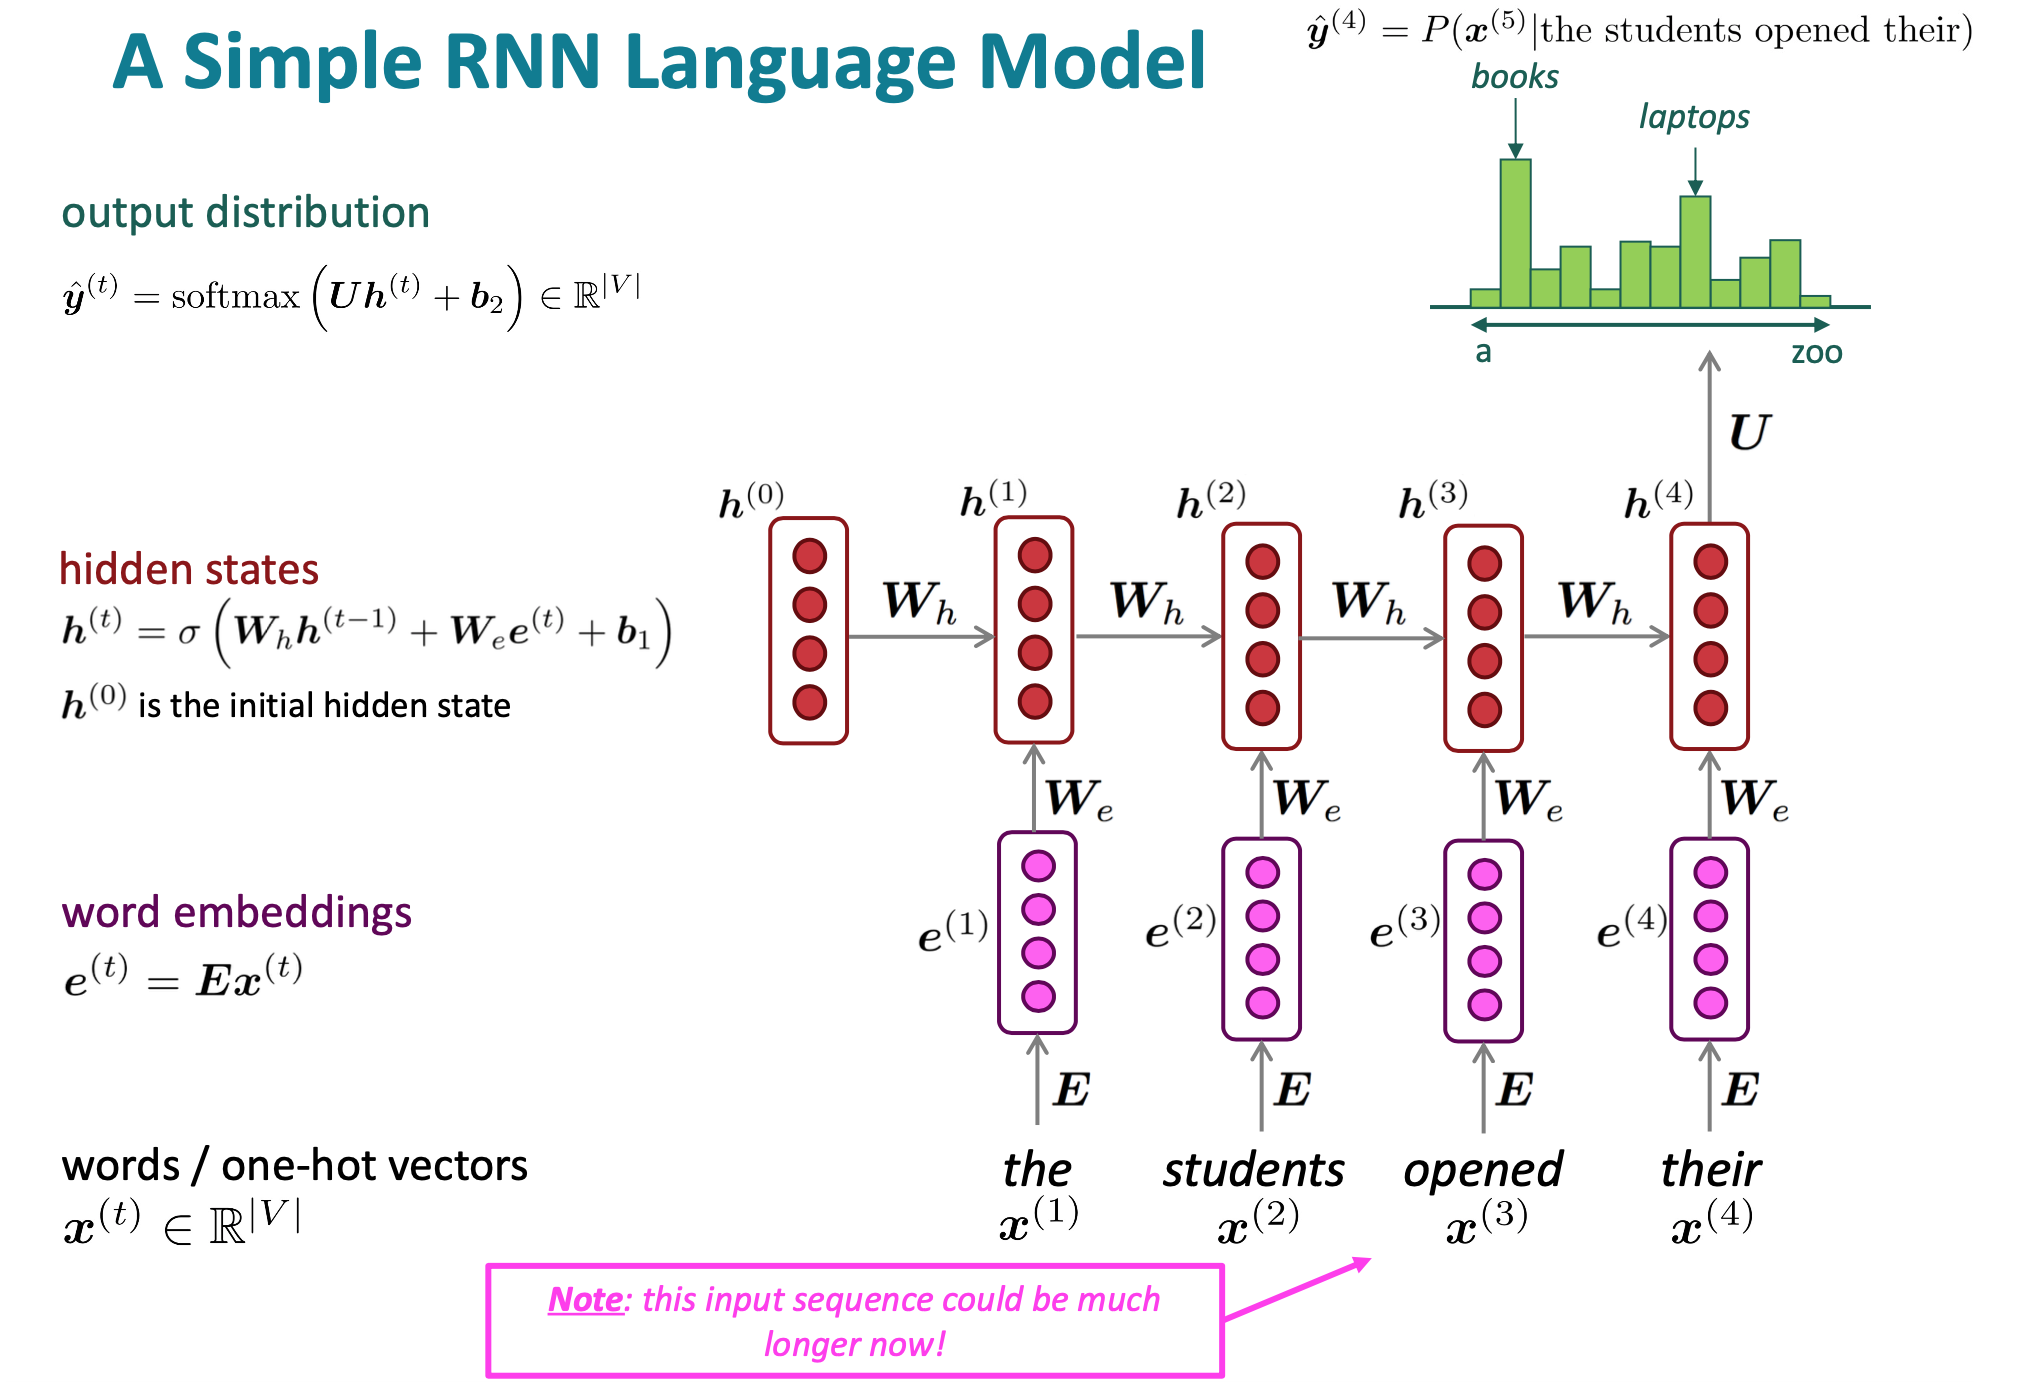
\includegraphics[height=2.2in, width=4.0in, viewport=0 0 1010 700,clip]{Figures/RNN-Language-model.png}
%\caption{\tiny \textrm{Pseudopotential for metallic sodium, based on the empty core model and screened by the Thomas-Fermi dielectric function.}}%(与文献\cite{EPJB33-47_2003}图1对比)
\label{RNN-language-model}
\end{figure}
\end{frame}

\begin{frame}
	\frametitle{\textrm{CNN}在\textrm{CV}中的基本思想}
	\textcolor{purple}{卷积神经网络~\textrm{(Convolutional Neural Network,~CNN)}}
\begin{figure}[h!]
\vspace*{-0.05in}
\centering
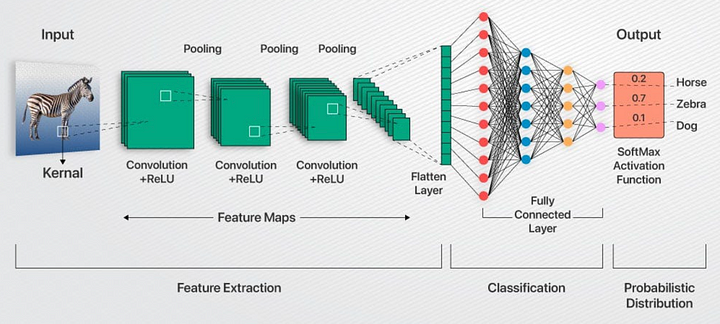
\includegraphics[height=1.9in, width=4.0in, viewport=0 0 720 324,clip]{Figures/CNN-CV-model.png}
%\caption{\tiny \textrm{Pseudopotential for metallic sodium, based on the empty core model and screened by the Thomas-Fermi dielectric function.}}%(与文献\cite{EPJB33-47_2003}图1对比)
\label{CNN-CV-model}
\end{figure}
\end{frame}

\begin{frame}
	\frametitle{\textrm{CNN}在\textrm{NLP}中的基本思想}
    \begin{itemize}
		\setlength{\itemsep}{10pt}
		\item 局部特征提取:~把文本中的每个单词类比为图像中的像素,\textrm{CNN}使用卷积核在文本序列上滑动,提取相邻单词组成的局部片段特征\\
			{\fontsize{7.2pt}{6.2pt}\selectfont{多个不同大小的卷积核能够提取多种尺度的特征,捕捉单词间的局部语义关系}}
        \item 特征整合与分类:~通过池化层对卷积得到的特征进行降维,整合局部特征,\textrm{CNN}获取文本的全局特征表示,进而用于文本分类、情感分析等任务\\
		{\fontsize{7.2pt}{6.2pt}\selectfont{例如在情感分析中,通过卷积和池化操作提取文本特征,再经全连接层判断文本表达的情感倾向}}
    \end{itemize}
    \textcolor{blue}{\textrm{CNN}:~通过卷积核在数据上滑动来提取局部特征,具备平移不变性,在图像识别等领域取得了显著成果}\\
    \vskip 2pt
    {\fontsize{8.2pt}{6.2pt}\selectfont{\textrm{CNN}的感受范围通常是局部的,可以通过堆叠多层卷积来扩大感受范围}}
\end{frame}

\section{从神经网络到\rm{Transformer}}
\begin{frame}
	\frametitle{传统神经网络方法的局限}
    在自然语言处理\textrm{(NLP)}和计算机视觉\textrm{(CV)}等诸多人工智能领域,循环神经网络\textrm{(RNN)}与卷积神经网络\textrm{(CNN)}曾占据主导地位\\
    {\fontsize{7.2pt}{6.2pt}\selectfont{\textcolor{red}{随着数据规模的增长和任务复杂度的提升,传统神经网络在长距离依赖和并行计算方面的局限性逐渐凸显}}}
    \begin{itemize}
	    \item \textrm{RNN}长距离依赖难题:~实际训练中,由于梯度消失或梯度爆炸问题,\textrm{RNN}很难学习到远距离的信息,\\
		    {\fontsize{7.2pt}{6.2pt}\selectfont{\textcolor{red}{例如:~在文本翻译任务中,开头的单词信息很难传递到句子末尾}}}\\
		    \textrm{RNN}的循环结构无法充分利用硬件的并行计算能力,大大增加了训练时间
	    \item \textrm{CNN}通过堆叠多层卷积来扩大感受范围,获取长距离依赖信息的效率较低\\
		    {\fontsize{7.2pt}{6.2pt}\selectfont{\textcolor{red}{比如:~在处理长文本时,难以直接捕捉到相隔较远的文本片段之间的语义关联}}}\\
		    虽然\textrm{CNN}在一定程度上可以并行计算,但由于卷积操作的局部特性,在捕捉全局依赖关系时,计算资源的浪费较为严重
    \end{itemize}
\end{frame}


\begin{frame}
	\frametitle{\textrm{Transformer}架构总览}
	\textrm{Transformer}于\textrm{2017}年%在论文《Attention Is All You Need》中被
    提出,放弃了\textrm{RNN}和\textrm{CNN}的序列结构与卷积操作,完全基于注意力机制\\
    {\fontsize{7.2pt}{6.2pt}\selectfont{在长文本处理、并行计算上表现卓越,迅速成为\textrm{NLP}的主流模型}}
\begin{figure}[h!]
%\vspace*{-0.15in}
\centering
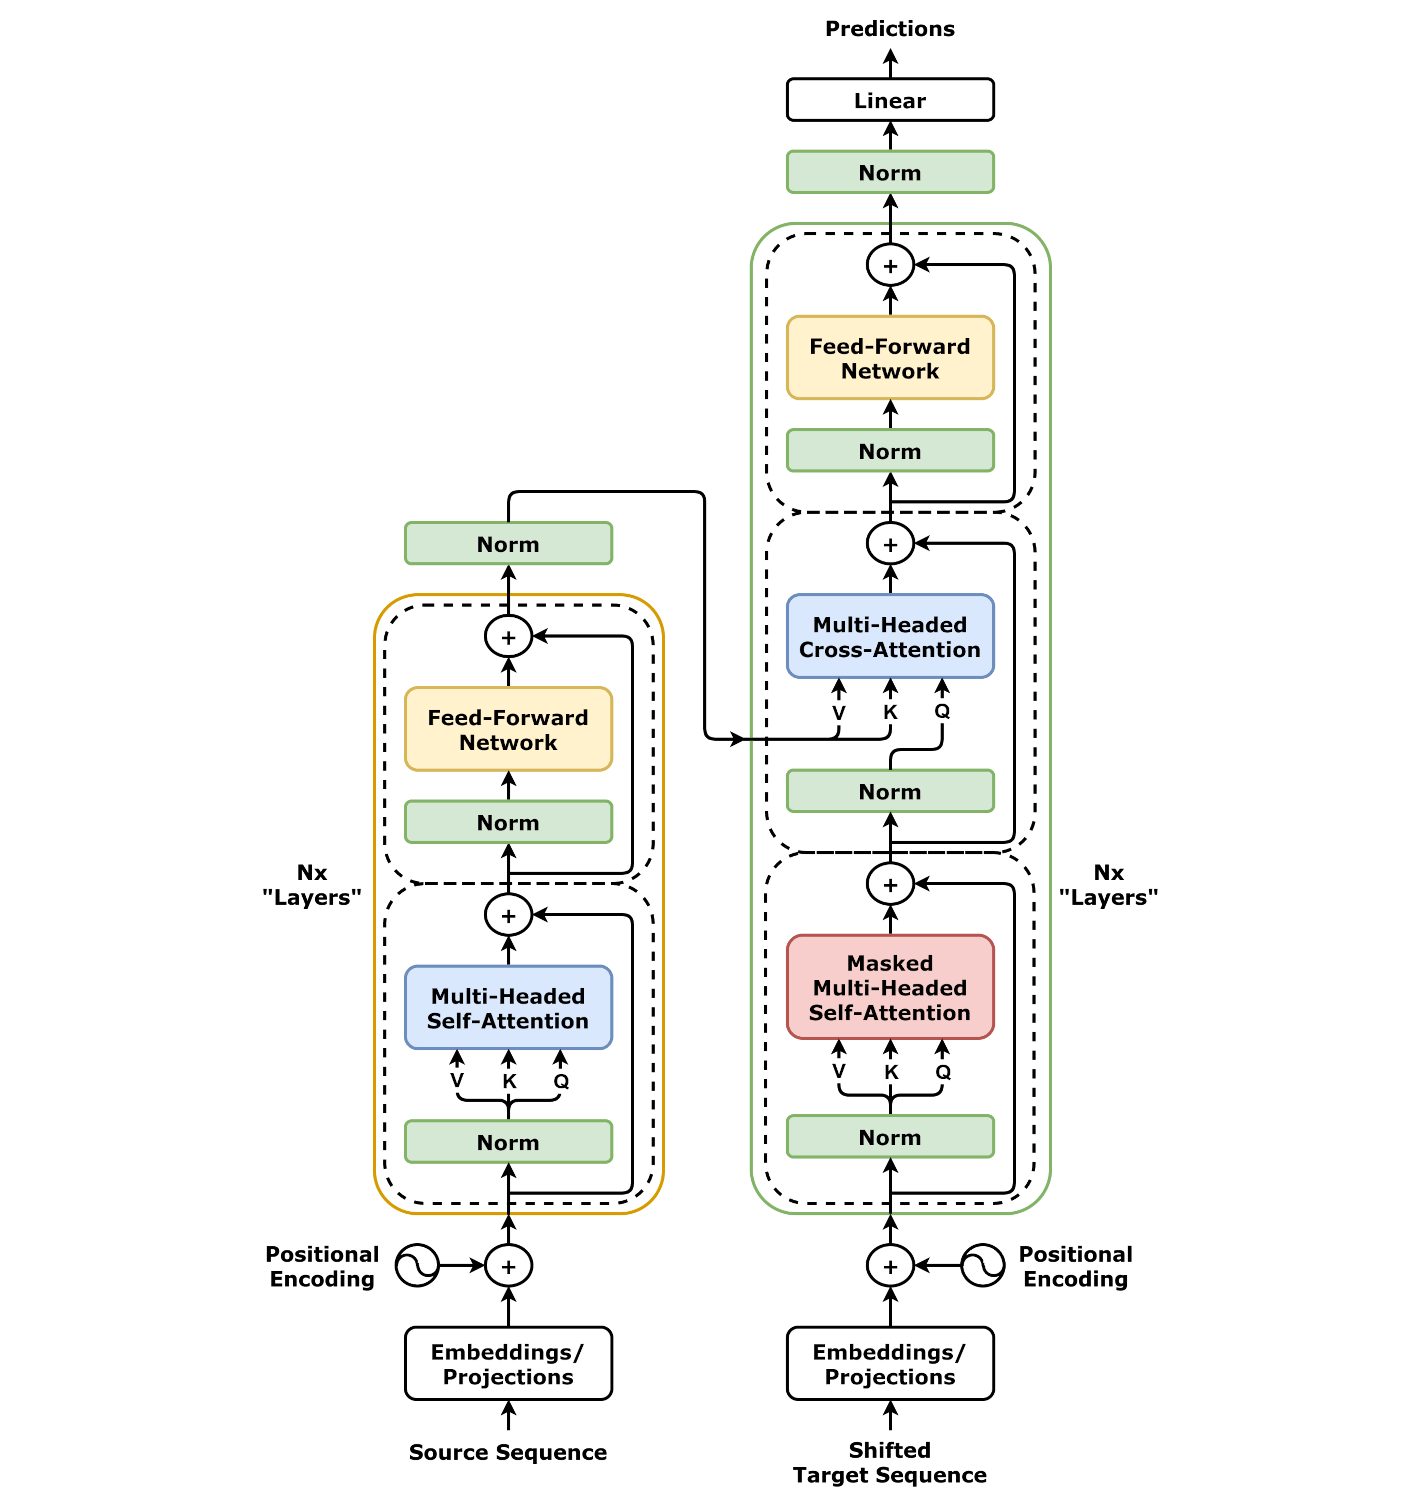
\includegraphics[height=2.0in, width=1.8in, viewport=300 0 1200 1500,clip]{Figures/Transformer_full_architecture.png}
\caption{\tiny \textrm{Transformer:~full architecture.}}%(与文献\cite{EPJB33-47_2003}图1对比)
\label{Transformer_full_architecture}
\end{figure}
\end{frame}

\begin{frame}
	\frametitle{\textrm{Transformer}的并行特点}
\begin{itemize}
	\item \textrm{Transformer}由编码器\textrm{(Encoder)}和解码器\textrm{(Decoder)}组成,分别包含多个相同的层,层间使用残差连接和归一化操作\\
    {\fontsize{7.2pt}{6.2pt}\selectfont{这样的模块设计,为并行计算提供了基础}}
    \item 在\textrm{Transformer}中,编码器和解码器内的多个层并非按顺序逐一计算,而是可以并行处理\\
	    {\fontsize{7.2pt}{6.2pt}\selectfont{在编码器中每个编码器层相互独立,在计算时,所有编码器层可以同时处理输入数据的不同部分,大幅提升计算效率}}
\end{itemize}
\begin{figure}[h!]
\vspace*{-0.05in}
\centering
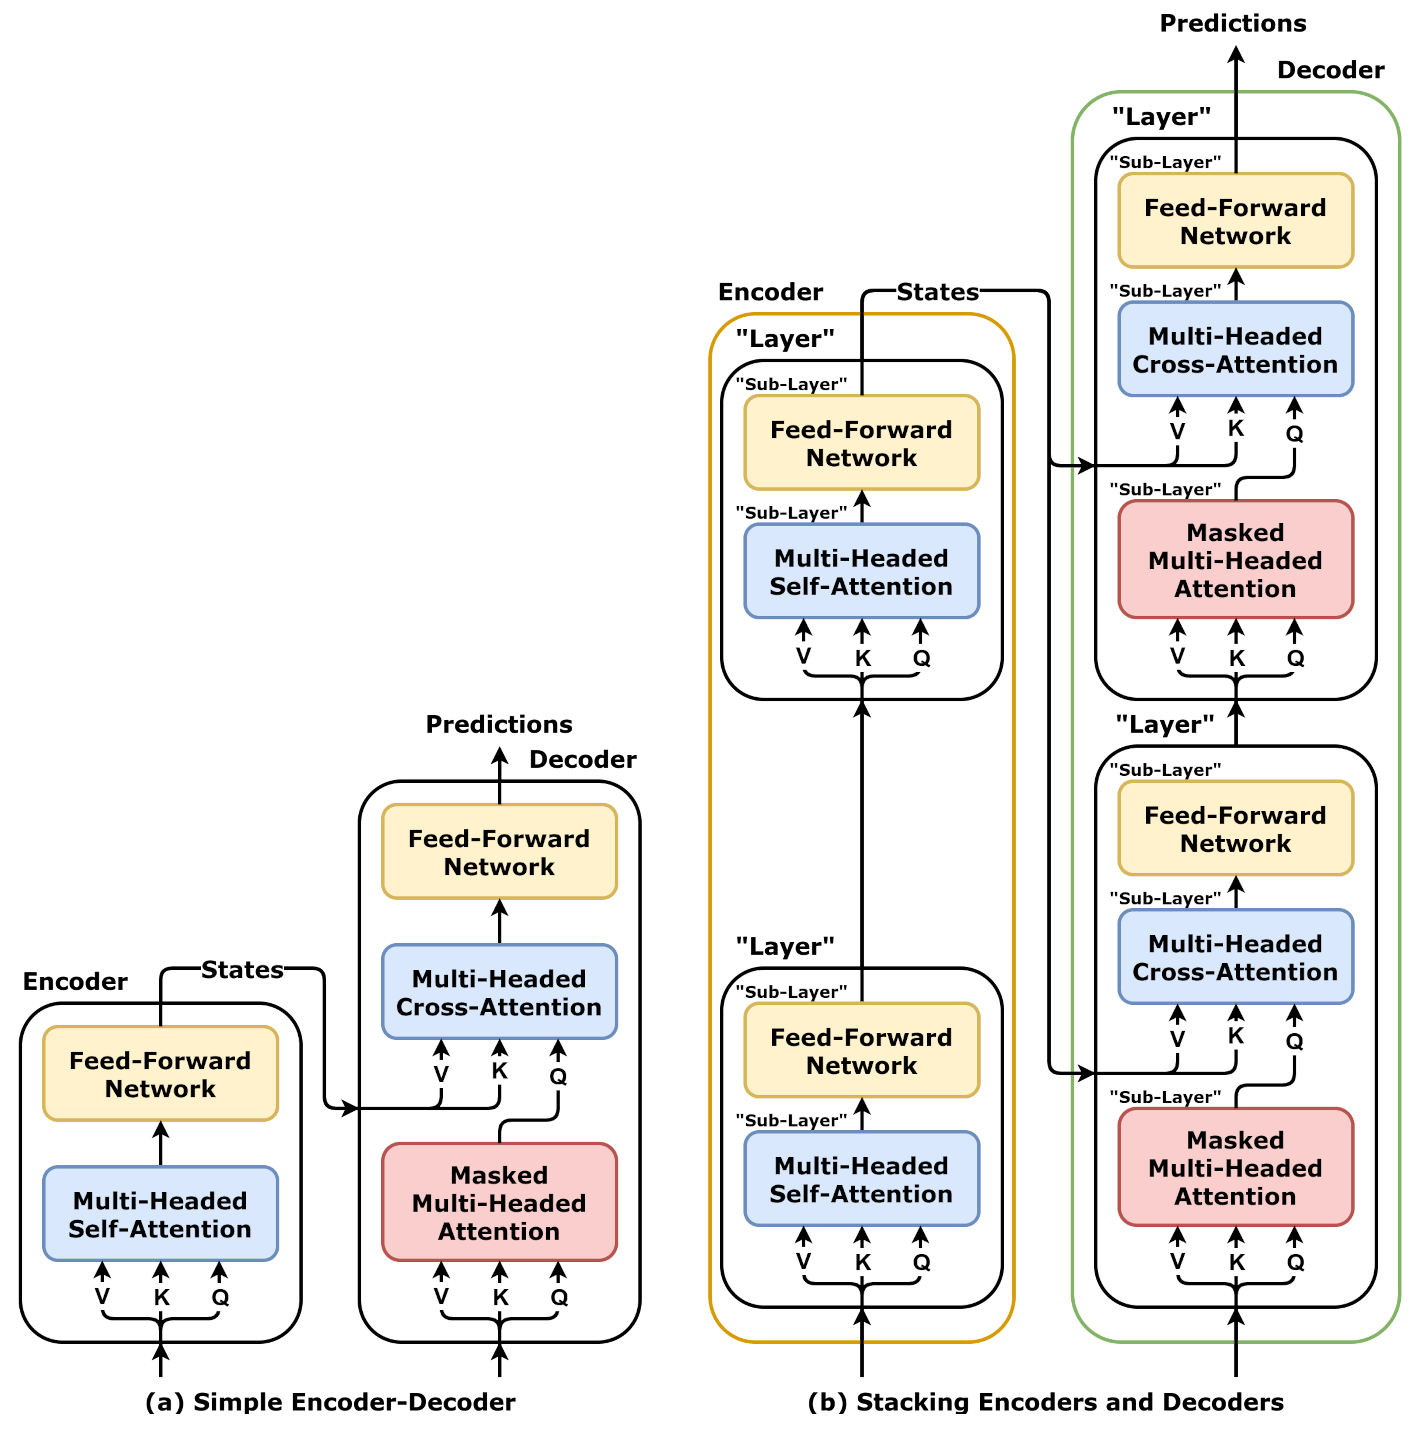
\includegraphics[height=1.5in, width=1.5in, viewport=0 0 1426 1430,clip]{Figures/Transformer_stacked_multilayers.png}
\caption{\tiny \textrm{Transformer:~stacked multilayers architecture.}}%(与文献\cite{EPJB33-47_2003}图1对比)
\label{Transformer_stacked_multilayers}
\end{figure}
\end{frame}

\section{\rm{Transformer}的主要技术}
\begin{frame}
    \frametitle{多头注意力机制中的并行计算}
    \textcolor{red}{多头注意力~\textrm{(Multi-Headed Self-Attention):}}\\
    允许模型在不同的表示子空间中并行地学习相关信息
    \begin{itemize}
	    \item 计算步骤:~\\
		    \begin{enumerate}
			    \item {\fontsize{7.2pt}{6.2pt}\selectfont{输入的查询\textrm{(Query)}、键\textrm{(Key)}和值\textrm{(Value)}分别经过线性变换得到多个不同的子查询、子键和子值:~}}{\fontsize{5.2pt}{4.2pt}\selectfont{\textcolor{magenta}{由于各子查询、子键、子值的线性变换相互独立,这些操作可以并行执行}}}
			    \item {\fontsize{7.2pt}{6.2pt}\selectfont{计算子查询与子键的点积注意力分数,并通过\textrm{Softmax}进行归一化}}
			    \item {\fontsize{7.2pt}{6.2pt}\selectfont{将加权后的子值进行拼接,并通过一个线性层得到最终的输出}}
    \end{enumerate}
	{\fontsize{7.2pt}{6.2pt}\selectfont{对于第$i$个注意力头,有:~
		    \begin{displaymath}
			    \mathrm{Attention}_i(Q, K, V) = \mathrm{Softmax}(\frac{Q W_i^Q (K W_i^K)^T}{\sqrt{d_k}}) V W_i^V 
		    \end{displaymath}
		    {\fontsize{5.2pt}{4.2pt}\selectfont{其中$W_i^Q$, $W_i^K$, $W_i^V$是可学习的权重矩阵,$d_k$是键向量的维度}}}}
        \item 多注意力头整合:
		\vskip 1pt
		{\fontsize{7.2pt}{6.2pt}\selectfont{将多个注意力头的输出拼接后,再经过一个线性变换,得到最终的多头注意力输出
		\begin{displaymath}
			\mathrm{MultiHead}(Q, K, V) = \mathrm{Concat}(\mathrm{Attention}_1, \cdots, \mathrm{Attention}_h) W^O
		\end{displaymath}
		多个注意力头之间的计算过程相互独立,能够同时进行}}
    \end{itemize}
\end{frame}

\begin{frame}
    \frametitle{多头注意力机制中的并行计算}
\begin{figure}[h!]
\vspace*{-0.15in}
\centering
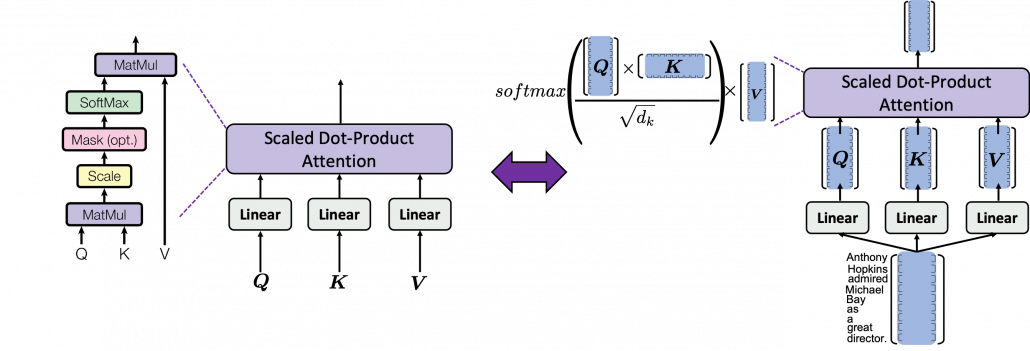
\includegraphics[height=1.3in, width=4.0in, viewport=0 0 800 300,clip]{Figures/MHA-scaled_dot_product.png}
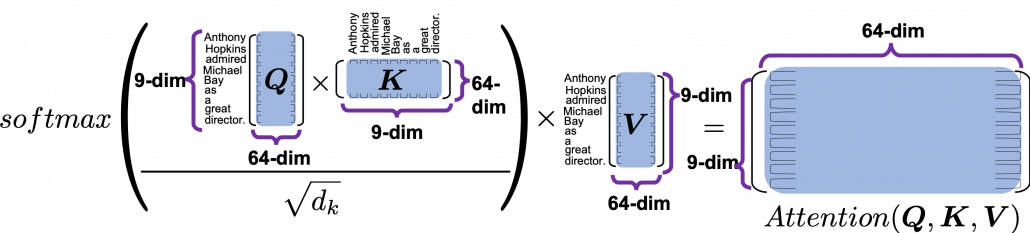
\includegraphics[height=0.8in, width=4.0in, viewport=0 0 800 193,clip]{Figures/MHA-scaled_dot_attention.png}
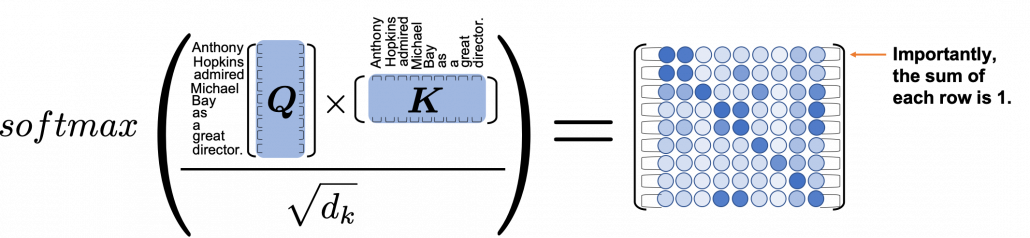
\includegraphics[height=0.8in, width=4.0in, viewport=0 0 800 200,clip]{Figures/MHA-self_attention_map.png}
%\caption{\tiny \textrm{Transformer:~stacked multilayers architecture.}}%(与文献\cite{EPJB33-47_2003}图1对比)
\label{Transformer_multiHead}
\end{figure}
\end{frame}

\begin{frame}
    \frametitle{前馈神经网络中的并行计算}
\textcolor{red}{前馈神经网络~\textrm{(Feed-Forward Network):}}\\
    在每个位置上独立运行,对注意力机制的输出,作出进一步处理
    \begin{itemize}
		\setlength{\itemsep}{3pt}
	    \item 结构:~包含两个线性变换层,中间使用\textrm{ReLU}作为激活函数
\begin{figure}[h!]
\vspace*{-0.05in}
\centering
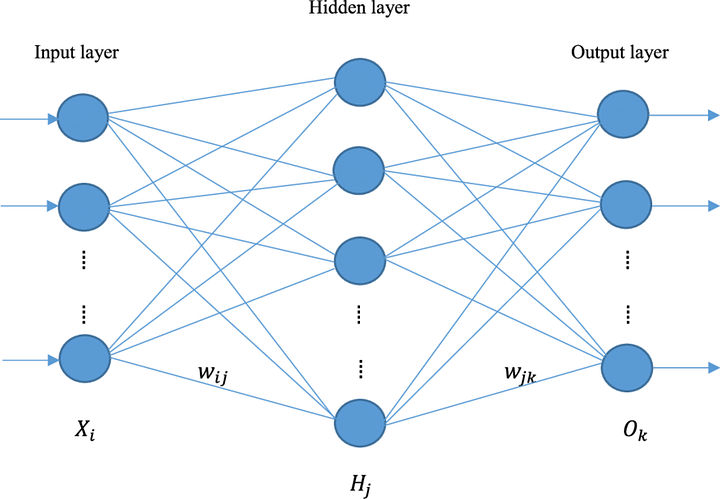
\includegraphics[height=1.1in, width=1.7in, viewport=0 0 720 499, clip]{Figures/Transformer_FFNN.png}
%\caption{\tiny \textrm{Transformer:~stacked multilayers architecture.}}%(与文献\cite{EPJB33-47_2003}图1对比)
\label{Transformer_FFNN}
\end{figure}
%		    数学表达式为
		    \begin{displaymath}
			     \mathrm{FFN}(x) = \max(0, x W_1 + b_1) W_2 + b_2 
		    \end{displaymath}
		    {\fontsize{7.2pt}{6.2pt}\selectfont{其中$W_1$, $W_2$是权重矩阵,$b_1$, $b_2$是偏置向量}}
%\vskip 2pt
{\fontsize{7.2pt}{6.2pt}\selectfont{\textcolor{magenta}{由于不同位置的输入在\textrm{FFN}中的计算彼此独立,因此可对整个序列并行计算}}}
        \item 作用:~为模型引入非线性变换,增强模型的表达能力,捕捉更复杂的模式
    \end{itemize}
\end{frame}

\begin{frame}
    \frametitle{解码器中的并行特性}
    解码器同样由多个解码器层堆叠而成
    \begin{itemize}
		\setlength{\itemsep}{10pt}
		\item 与编码器不同,解码器层在多头注意力机制前多了一个\textcolor{blue}{掩码多头注意力机制}
		\item \textcolor{purple}{掩码多头注意力机制需要按顺序生成序列}
		\item 在每个时间步内,\textcolor{blue}{掩码多头注意力机制}与\textcolor{purple}{交叉注意力机制}的计算,以及\textcolor{magenta}{前馈神经网络}的运算,都可以并行完成
    \end{itemize}
\end{frame}

\begin{frame}
    \frametitle{掩码多头注意力机制的并行}
\textcolor{red}{掩码多头注意力~\textrm{(Masked Multi-Headed Self-Attention):}}
    \begin{itemize}
		\setlength{\itemsep}{10pt}
        \item 掩码操作:~在计算注意力分数时,通过掩码矩阵屏蔽未来位置的信息,保证模型在训练时不会“偷看”未来的输入
		\vskip 1pt
		{\fontsize{7.2pt}{6.2pt}\selectfont{掩码矩阵是一个上三角矩阵,对角线及以下元素为\textrm{0},对角线以上元素为负无穷\\
		经过\textrm{Softmax}后,未来位置的注意力分数为\textrm{0}}}
        \item 防止信息泄露:~确保了模型在推理过程中,只能依赖当前及之前的信息,符合自然语言处理的因果关系
	\item 尽管要遵循顺序生成的原则,但在计算\textcolor{red}{同一时刻的注意力分数}时,各位置间的运算依然可以并行
    \end{itemize}
\begin{figure}[h!]
\vspace*{-0.05in}
\centering
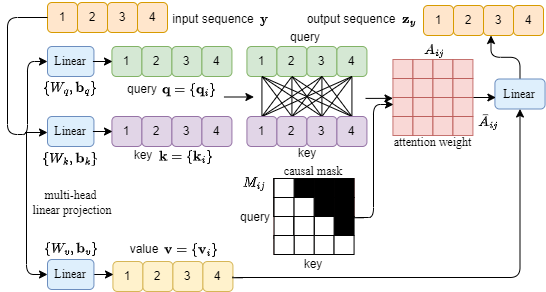
\includegraphics[height=0.9in, width=1.8in, viewport=0 0 546 292, clip]{Figures/Masked_multi-head_self-attention-for-a-target_sequence-y.png}
%\caption{\tiny \textrm{Transformer:~stacked multilayers architecture.}}%(与文献\cite{EPJB33-47_2003}图1对比)
\label{Masked_multi-head_self-attention-for-a-target_sequence-y}
\end{figure}
\end{frame}

\begin{frame}
    \frametitle{交叉注意力机制的并行}
\begin{figure}[h!]
\vspace*{-0.15in}
\centering
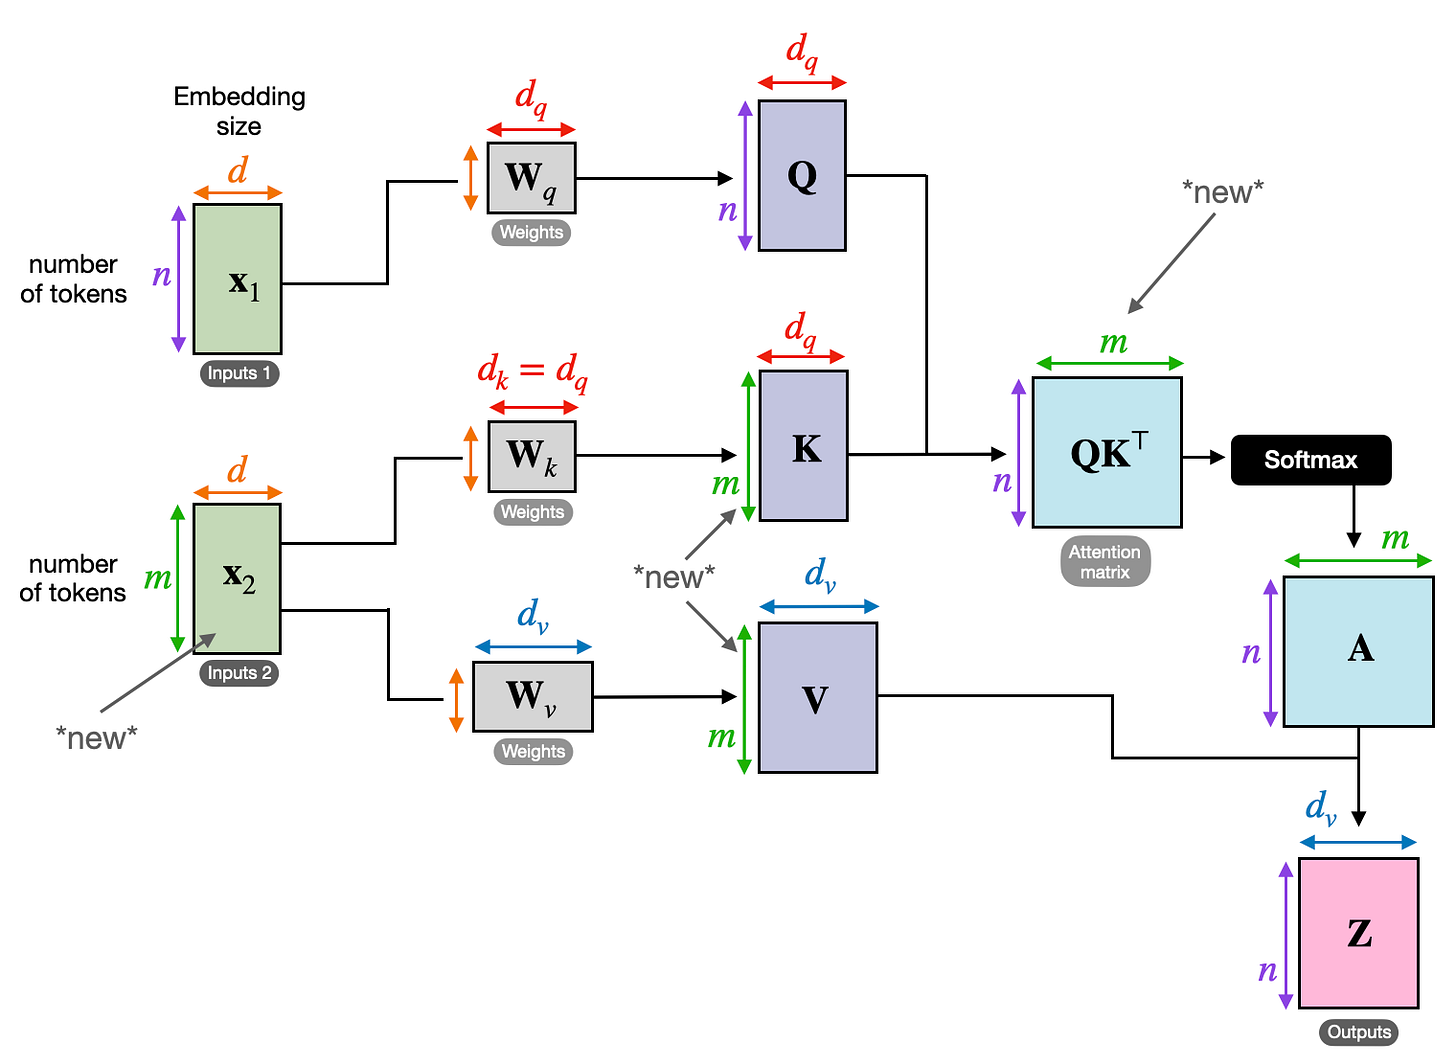
\includegraphics[height=2.7in, width=3.8in, viewport=0 0 1456 1061, clip]{Figures/Transformer_The_concept_of_cross-attention.png}
%\caption{\tiny \textrm{Transformer:~stacked multilayers architecture.}}%(与文献\cite{EPJB33-47_2003}图1对比)
\label{Transformer_The_concept_of_cross-attention}
\end{figure}
\end{frame}

\begin{frame}
    \frametitle{交叉注意力机制的并行}
\textcolor{red}{交叉注意力~\textrm{(Multi-Headed Cross-Attention):}}\\
以编码器的输出作为键和值
    \begin{itemize}
		\setlength{\itemsep}{10pt}
        \item 信息交互:~以解码器上一层的输出作为查询
\vskip 1pt
		{\fontsize{7.2pt}{6.2pt}\selectfont{通过计算注意力分数,解码器可以从编码器的输出中获取相关的上下文信息}}
	\item 交叉注意力机制在计算时,不同位置的查询向量,键、值向量的运算,可并行进行
        \item 交叉注意力计算过程与多头注意力机制类似,只是查询、键和值的来源不同
	\item 交叉注意力机制帮助解码器聚焦于输入序列的不同部分,从而更好地生成输出
    \end{itemize}
\end{frame}

\begin{frame}
	\frametitle{与\textrm{RNN}、\textrm{CNN}的对比}
	\renewcommand{\arraystretch}{1.1} % 调整整体行间距
    \begin{table}[ht]
        \centering
        \begin{tabular}{lll}
    \toprule
	    特性 & \textrm{RNN} & \textrm{Transformer} \\
            \midrule
            结构 & 循环结构,顺序处理数据 & 并行处理数据 \\
            \hline
	    \multirow{2}{*}{长距离依赖} & 梯度消失或崩溃, & 自注意力机制, \\
		    &难以处理长距离依赖 &有效捕捉长距离依赖 \\
            \hline
            计算效率 & 顺序计算,效率低 & 并行计算,效率高 \\
            \bottomrule
        \end{tabular}
	\caption{\tiny{\textrm{RNN}与\textrm{Transformer}的对比}}
    \end{table}
    \vskip -13pt
    \begin{table}[ht]
        \centering
        \begin{tabular}{lll}
    \toprule
	    特性 & \textrm{CNN} & \textrm{Transformer} \\
            \midrule
	    \multirow{2}{*}{感受域} & 局部感受范围,& 全局感受域,\\
	    & 通过堆叠扩大感受域 & 自注意力机制获取全局信息 \\
            \hline
            归纳偏置 & 平移不变性,局部连接 & 无特定归纳偏置 \\
            \hline
	    应用场景 & 图像领域表现出色 & \textrm{NLP}领域表现出色 \\
            \bottomrule
        \end{tabular}
	\caption{\tiny{\textrm{CNN}与\textrm{Transformer}的对比}}
    \end{table}
\end{frame}

%\begin{frame}
%    \frametitle{总结}
%    \textrm{Transformer}凭借自注意力机制和精心设计的架构,实现了高效的并行计算,解决了长距离依赖和并行计算的问题,在\textrm{NLP}领域取得了巨大成功\\
%
%    它不仅革新了\textrm{NLP}研究,也推动了其他领域如计算机视觉的发展,未来有望在更多领域发挥重要作用
%\end{frame}
